\documentclass[10pt, conference, compsocconf]{IEEEtran}

\hyphenation{data-bases}
\newcommand{\Comet}{{\em Comet\/}}

\newcommand{\TITLE}{Virtual Cluster management for Heterogeneous Cloud Platforms}
\newcommand{\AUTHOR}{Gregor von Laszewski, Fugang Wang, Badi Abduhl Wahid, Hyungro Lee}

%%%%%%%%%%%%%%%%%%%%%%%%%%%%%%%%%%%%%%%%%%%%%%%%%%%%%%%%%%%%%%
% LATEX DEFINITIONS 
%%%%%%%%%%%%%%%%%%%%%%%%%%%%%%%%%%%%%%%%%%%%%%%%%%%%%%%%%%%%%%

\usepackage{float}
\usepackage{comment}
\usepackage{hyperref} 
\usepackage{array} 
\usepackage{graphicx} 
\usepackage{booktabs} 
\usepackage{pifont} 
\usepackage{todonotes} 
\usepackage{rotating} 
\usepackage{color} 
\usepackage{caption}
\captionsetup{font={scriptsize}}

\newcommand*\rot{\rotatebox{90}} 
 
\newcommand{\FILE}[1]{\todo[color=green!40]{#1}} 
 

%
% more floats on one page
%
\renewcommand{\topfraction}{.85}
\renewcommand{\bottomfraction}{.7}
\renewcommand{\textfraction}{.15}
\renewcommand{\floatpagefraction}{.66}
\renewcommand{\dbltopfraction}{.66}
\renewcommand{\dblfloatpagefraction}{.66}
\setcounter{topnumber}{9}
\setcounter{bottomnumber}{9}
\setcounter{totalnumber}{20}
\setcounter{dbltopnumber}{9}

%%%%%%%%%%%%%%%%%%%%%%%%%%%%%%%%%%%%%%%%%%%%%%%%%%%%%%%%%%%%%%
% HYPERSETUP 
%%%%%%%%%%%%%%%%%%%%%%%%%%%%%%%%%%%%%%%%%%%%%%%%%%%%%%%%%%%%%%

\hypersetup{ 
    bookmarks=true,         % show bookmarks bar 
    unicode=false,          % non-Latin characters in Acrobat's bookmarks 
    pdftoolbar=true,        % show Acrobat's toolbar 
    pdfmenubar=true,        % show Acrobat's menu 
    pdffitwindow=false,     % window fit to page when opened 
    pdfstartview={FitH},    % fits the width of the page to the window 
    pdftitle={\TITLE},    % title 
    pdfauthor={\AUTHOR},     % author 
    pdfsubject={Subject},   % subject of the document 
    pdfcreator={Gregor von Laszewski, Fugang Wang},   % creator of the document 
    pdfproducer={}, % producer of the document 
    pdfkeywords={hindex} {metric}{XSEDE} {FutureGrid}, % list of keywords 
    pdfnewwindow=true,      % links in new window 
    colorlinks=false,       % false: boxed links; true: colored links 
    linkcolor=red,          % color of internal links (change box color with linkbordercolor) 
    citecolor=green,        % color of links to bibliography 
    filecolor=magenta,      % color of file links 
    urlcolor=cyan           % color of external links 
} 

\begin{document}

\begin{comment}
%\conferenceinfo{submitted to XSEDE}{'15,  July 26 - 30 2015, St. Louis, MO, USA}
\conferenceinfo{submitted to ...}{2015,USA}
\CopyrightYear{2015} 
\crdata{TBD...\$15.00.\\
http://dx.doi.org/TBD
} 
\end{comment}

\title{\TITLE\vspace{-12pt}}


\author{\IEEEauthorblockN{%
Gregor von Laszewski,
Fugang Wang,
Badi Abduhl Wahid,
Hyungro Lee,
Geoffrey C. Fox, }
\IEEEauthorblockA{%
$^1$School of Informatics and Computing, Indiana University, Bloomington, Indiana, U.S.A.\\ 
laszewski@gmail.com}
}

\maketitle

\begin{abstract}

TBD

\end{abstract}

\begin{comment}
\vspace{-6pt}


\category{H.4}{Information Systems Applications}{Miscellaneous}
\category{D.2.8}{Software Engineering}{Metrics}[complexity measures,
performance measures]

\terms{Theory, Measurement}

\keywords{Scientific impact, bibliometric, h-index, Technology Audit
  Service, XDMoD, XSEDE}
\end{comment}

\section{Introduction} 


\begin{figure}[htb] 
  \centering 
    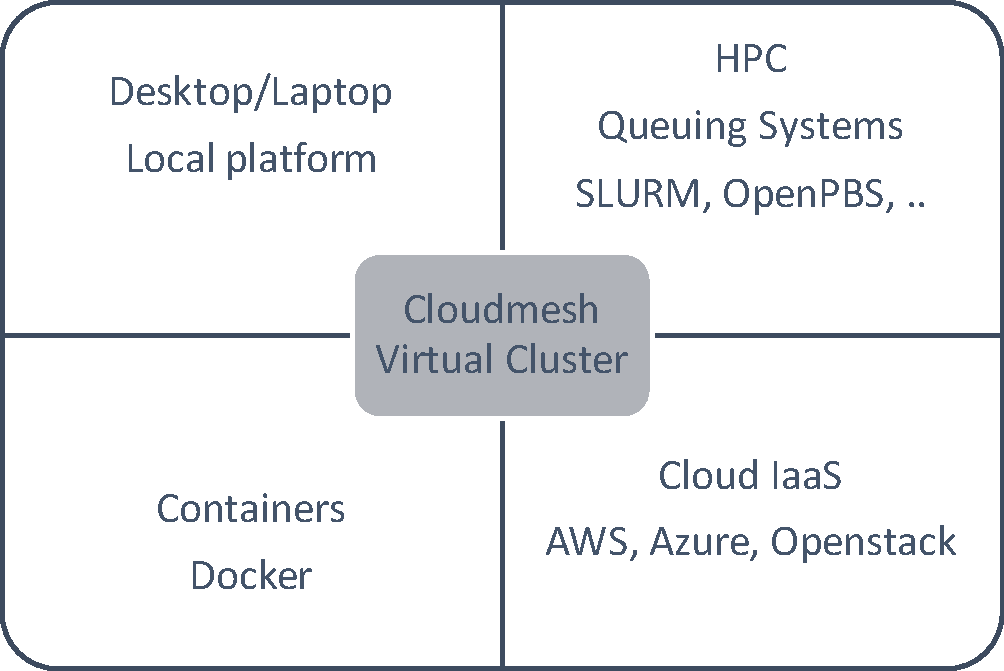
\includegraphics[width=1.0\columnwidth]{images/cm-machines.pdf} 
    \caption{Basic compute resource abstraction of cloudmesh}
    \label{F:objectives}
\end{figure} 

\begin{figure}[htb] 
  \centering 
    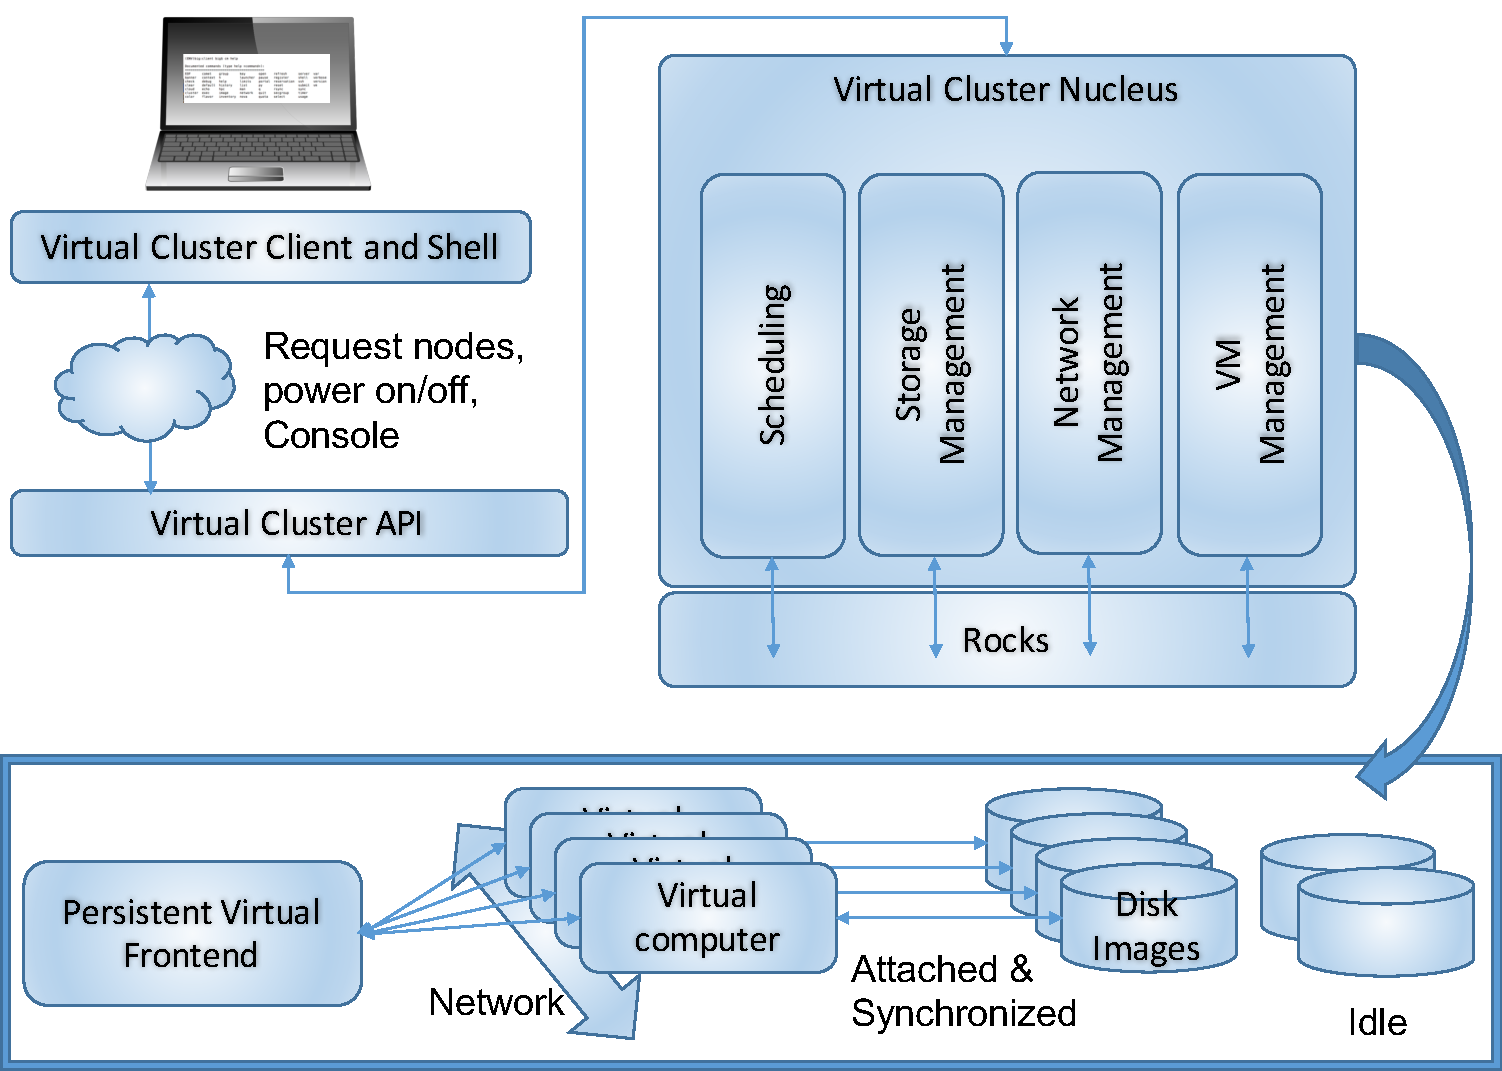
\includegraphics[width=1.0\columnwidth]{images/comet-arch.pdf} 
    \caption{High level Objectives impacting the design of our framework}
    \label{F:objectives}
\end{figure} 


\section{Related Work} \label{S:related}

\section{Design}

\subsection{Requirements}


\subsection{Architecture}


\begin{comment}

SAMPLE IMAGE

\begin{figure}[htb] 
  \centering 
    \includegraphics[width=1.0\columnwidth]{images-new/objectives.pdf} 
    \caption{High level Objectives impacting the design of our framework}
    \label{F:objectives}
\end{figure} 

\end{comment}

\section{Analysis}




\subsection{Hybrid Cloud Achievement}


Comet has easy to use CLI allowing the use of Comet as infrastructure for virtual cluster management.


Cloudmesh has more functionality:
\begin{itemize}
\item Access hybrid clouds OpenStack, (EC2, AWS, Azure) Access
  concrete
\item infrastructure demonstrated usages of FutureSystems, Chameleon,
\item CloudLab, Cybera (CA) Once we get access: Bridges, Jetstream, ...
\item (EC2, AWS, Azure)
\end{itemize}
A user could use all of them

\subsection{Motivation}

Users are flexible and can chose the infrastructure most suitable for a particular problem while accessing them through the same client.  Switching from one infrastructure to another is simple while using templates and defaults

\begin{verbatim}
cm var cloud=jetstream / bridges / aws / ...
cm default cloud=$cloud
cm boot
\end{verbatim}

Rich Platform Stacks to Enable Reusable Virtual Cluster Templates

\begin{itemize}
\item Leverage from open source and proprietary services and tools
\item Pick the one most suitable
\item Integrate in DevOps
\item Make available through Cloudmesh launchers
\end{itemize}
cloudmesh launcher

Example:Install a Compute Node


\subsection{Virtual Clusters}

\begin{itemize}
\item Successful Early Operations
\item Developed a functional cloud environment leveraging:
\item Existing Rocks virtual cluster features
\item IU's FutureGrid experience and Cloudmesh client
\item Our ability to integrate with the standard HPC environment
\item Successfully deployed OSG virtual cluster
\item Virtual cluster used for CAIDA BGP Hackathon 2016
\item Hardening features
\item On ramping new groups
\item Pushing virtual cluster capability further into Comet
\item Excitement and caution
\item Developing cluster templates (Generic HPC cluster, Big Data) via Cloudmesh Launchers
\end{itemize}

\subsection{Other achievements}
\begin{itemize}
\item Pioneering XSEDE Cloud Allocation and Accounting
\item Virtual clusters use compute nodes as building blocks
\item Allocated based on compute SUs
\item Usage tracked based on compute SUs
\item XDMoD adding cloud utilization features via Open XDMoD
\item Builds on hardware resource utilization from TACC Stats
\item Needed for Comet, Jetstream, future XSEDE cloud systems
\item Need to have ongoing conversation with early users about \item reporting
\item Should projects report back like gateways?
\item Users, jobs, etc.?
\item Projects will likely need to track for subsequent XRACs \item regardless
\item After OSG, Many New Projects Ready to Begin
\item User-Customized HPC
\item High Performance Virtual Cluster Characteristics
\item What About Data?
\item Local storage
\item Can use Seagate SSDs for large VM images
\item Local (SDSC) network access same as compute nodes
\item We provide modest (TB) storage via NFS now
\item Working on secure access to Lustre
\item Accessing Virtual Cluster Capabilities
\end{itemize}



\subsection{What is next: Platforms}

\begin{itemize}
\item Example: NIST BigData Working group
\item Gather use case input from all stakeholders 
\item Derive Big Data requirements from each use case.
\item Analyze/prioritize a list of challenging general requirements that may delay or prevent adoption of BigData deployment 
\item Work with Reference Architecture to validate requirements and reference architecture
\item Develop a set of general patterns capturing the {\em essence} of use cases (to do)
\item Rich Platform Stacks to Enable Reusable Virtual Cluster Templates
\item Leverage from open source and proprietary services and tools
\item Pick the one most suitable
\item Integrate in DevOps
\item Make available through Cloudmesh launchers
\end{itemize}

\subsection{Comet Cloudmesh Platform Launchers}

\begin{itemize}
\item Launch specific platform selections
\item Target Application user communities
\item Make deployment and management simple
\item Customizable launchers
\item Launchers available through commandline or browser
\item Underlying ZFS layer makes cloning cluster template trivial
\item Comet Cloudmesh Platform Launchers (Future)
\item Specific Launch
\item List of Launchers
\item Concepts, Ideas, Design
\end{itemize}

\subsection{Enabling Technologies}
\begin{description}
\item[KVM:] Let us run virtual machines (all processor features)
\item[SR-IOV:] Makes MPI go fast on VMs
\item[Rocks:] Systems management
\item[ZFS:] Disk image management
\item[VLANs:] Isolate virtual cluster management network
\item[pkeys:] Isolate virtual cluster IB network
\item[Nucleus:] Coordination engine (scheduling, provisioning, status,
  etc.)
\item[Cloudmesh:] The client to virtual cluster management is
  provided by cloudmesh 
\end{description}


\section{NIST Big Data Use Cases}

51 NIST Big Data Benchmark Detailed Use Cases

\subsection{Government Operation} 

National Archives and Records Administration, Census BureauCommercial:
Finance in Cloud, Cloud Backup, Mendeley (Citations), Netfilx, Web
Search, Digital Materials, Cargo shipping (as in UPS)Defense: Sensors,
Image surveillance, Situation AssessmentHealthcare and

\subsection{Life Sciences} 

Medical records, Graph and Probabilistic analysis, Pathology,
Bioimaging, Genomics, Epidemiology, People Activity models,
BiodiversityDeep Learning and Social Media: Driving Car, Geolocate
images/cameras, Twitter, Crowd Sourcing, Network Science, NIST
benchmark datasets

\subsection{The Ecosystem for Research} 

Metadata, Collaboration, Language Translation, Light source
experiments

\subsection{Astronomy and Physics} 

Sky Surveys compared to simulation, Large Hadron Collider at CERN,
Belle Accelerator II in JapanEarth,

\subsection{Environmental and Polar Science} 

Radar Scattering in Atmosphere, Earthquake, Ocean, Earth Observation,
Ice sheet Radar scattering, Earth radar mapping, Climate simulation
datasets, Atmospheric turbulence identification, Subsurface
Biogeochemistry (microbes to watersheds), AmeriFlux and FLUXNET gas
sensors

\subsection{Energy} 

SmartGrid infrastructure for virtual cluster management.



\begin{verbatim}
http://cloudmesh.github.io/client/reference_card.html#refcard-comet
http://cloudmesh.github.io/client/commands/command_comet.html#comet-command
\end{verbatim}


\subsection{Client Portal}

\begin{figure}[htb] 
  \centering 
    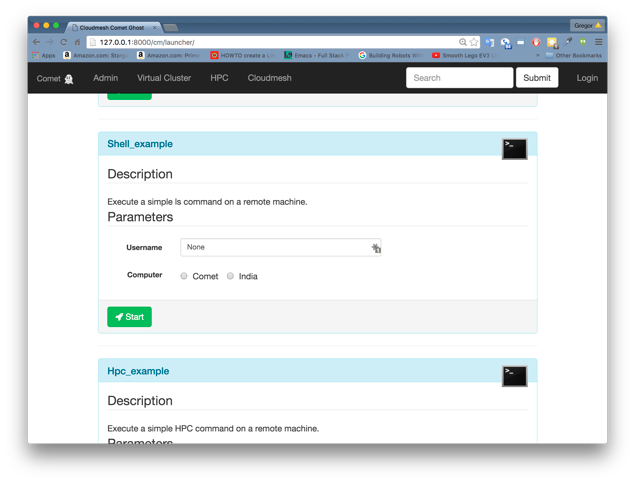
\includegraphics[width=1.0\columnwidth]{images/client/Picture6.png} 
    \caption{Virtual cluster launch parameters}
    \label{F:6}
\end{figure} 

\begin{figure}[htb] 
  \centering 
    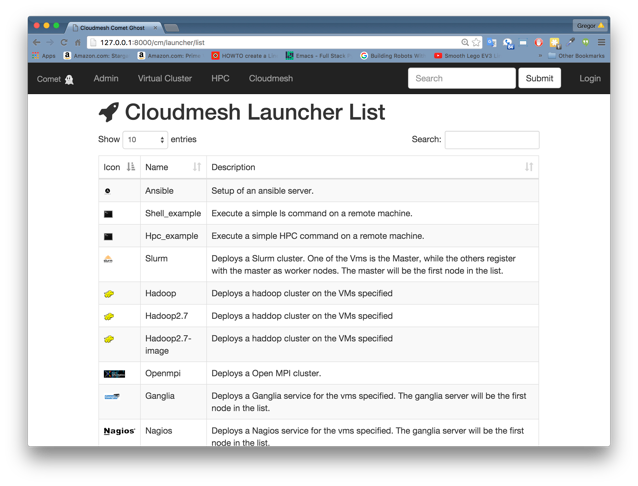
\includegraphics[width=1.0\columnwidth]{images/client/Picture7.png} 
    \caption{Virtual cluster launcher}
    \label{F:7}
\end{figure} 


\subsection{Form Tutorial}

\begin{figure*}[htb] 
\begin{small}
\begin{verbatim}

+------+---------+-------+------------------------------------------+---------------+------------+-----------+-------------+
| Name | Project | Count | Nodes                                    | Frontend (Fe) | State (Fe) | Type (Fe) | Description |
+------+---------+-------+------------------------------------------+---------------+------------+-----------+-------------+
| vc1  | sys200  | 8     | vc1-[0-7]                                | vc1           | nostate    | VM        |             |
| vc2  | iu      | 8     | vm-vc2-[0-7]                             | vc2           | active     | VM        |             |
| vc3  | sys200  | 16    | compute-0-[0-12,14],compute_windows_10,d | vc3           | active     | VM        |             |
|      |         |       | imm_dev_node                             |               |            |           |             |
| vc4  | iu      | 8     | tstfw[1-2],vm-vc4-[0-5]                  | vc4           | active     | VM        |             |
| vc5  | sys200  | 11    | vm-vc5-[0-10]                            | vc5           | nostate    | VM        |             |
| vc6  | rocks   | 8     | vm-vc6-[0-7]                             | vc6           | nostate    | VM        |             |
| vc8  | sys200  | 0     |                                          | vc8           | active     | VM        |             |
| osg  | osg     | 34    | vm-osg-[0-33]                            | osg           | active     | VM        |             |
+------+---------+-------+------------------------------------------+---------------+------------+-----------+-------------+
\end{verbatim}
\end{small}
\end{figure*}

\begin{figure*}[htb] 
\begin{small}
\begin{verbatim}

Comet Cloudmesh Client (cluster view)
(COMET)host:client$ cm comet cluster
Cluster: osg	Frontend: osg	IP: 10.21.255.180
Cluster: vc1	Frontend: vc1	IP: 10.21.255.182
.........
Cluster: vc8	Frontend: vc8	IP: 10.21.255.175
\end{verbatim}
\end{small}
\end{figure*}

\begin{figure*}[htb] 
\begin{small}
\begin{verbatim}


+--------------------+---------------+----------+------+-------------------+------+---------+--------+---------+------------+
| name               | state         | kind     | type | mac               | cpus | cluster | RAM(M) | disk(G) | computeset |
+--------------------+---------------+----------+------+-------------------+------+---------+--------+---------+------------+
| osg                | active        | frontend | VM   | ca:5f:a8:00:00:1b | 8    | osg     | 32768  | 36      |            |
|                    |               |          |      | ca:5f:a8:00:00:1c |      |         |        |         |            |
| vm-osg-0           | active        | compute  | VM   | ca:5f:a8:00:00:1d | 24   | osg     | 120000 | 100     | 1065       |
| vm-osg-1           | active        | compute  | VM   | ca:5f:a8:00:00:1e | 24   | osg     | 120000 | 100     | 1066       |
| vm-osg-2           | active        | compute  | VM   | ca:5f:a8:00:00:1f | 24   | osg     | 120000 | 100     | 1067       |
.........
| vm-vc6-6           | nostate       | compute  | VM   | ca:5f:a8:00:00:7a | 24   | vc6     | 120000 | 36      |            |
| vm-vc6-7           | nostate       | compute  | VM   | ca:5f:a8:00:00:7b | 24   | vc6     | 120000 | 36      |            |
| vc8                | active        | frontend | VM   | ca:5f:a8:00:00:6d | 2    | vc8     | 4096   | 160     |            |
|                    |               |          |      | ca:5f:a8:00:00:6e |      |         |        |         |            |
+--------------------+---------------+----------+------+-------------------+------+---------+--------+---------+------------+
\end{verbatim}
\end{small}
\end{figure*}

\begin{figure*}[htb] 
\begin{small}
\begin{verbatim}


Comet Cloudmesh Client (computeset view)
(COMET)host:client$ cm comet computeset --cluster=osg

ClusterID: osg	ComputesetID: 1065	 State: running		Allocation: sys200
Start (est): 03/29/16 16:55 EDT		End (est): 03/31/16 16:55 EDT
Requested Time (ddd-hh:mm): 2-00:00	Running Time (est): 1-19:23		Remaining Time (est): 04:36
+----------+--------+------+-------------------+------+---------+------+--------+
| name     | state  | type | mac               | cpus | cluster | host | memory |
+----------+--------+------+-------------------+------+---------+------+--------+
| vm-osg-0 | active | VM   | ca:5f:a8:00:00:1d | 24   | osg     |      | 120000 |
+----------+--------+------+-------------------+------+---------+------+--------+
\end{verbatim}
\end{small}
\end{figure*}

\begin{figure*}[htb] 
\begin{small}
\begin{verbatim}

ClusterID: osg	ComputesetID: 1066	 State: running		Allocation: sys200
Start (est): 03/29/16 17:00 EDT		End (est): 03/31/16 17:00 EDT
Requested Time (ddd-hh:mm): 2-00:00	Running Time (est): 1-19:17
Remaining Time (est): 04:42

+----------+--------+------+-------------------+------+---------+------+--------+
| name     | state  | type | mac               | cpus | cluster | host | memory |
+----------+--------+------+-------------------+------+---------+------+--------+
| vm-osg-1 | active | VM   | ca:5f:a8:00:00:1e | 24   | osg     |      | 120000 |
+----------+--------+------+-------------------+------+---------+------+--------+
\end{verbatim}
\end{small}
\end{figure*}

\begin{figure*}[htb] 
\begin{small}
\begin{verbatim}


Comet Cloudmesh Client (start new computeset)
(COMET)host:client$ cm comet start vc2 --count=2 --walltime=3h
Request accepted! Check status with:
comet cluster vc2
or:
comet computeset 1102
(COMET)host:client$ cm comet computeset 1102

(COMET)host:client$ cm comet start vc4 vm-vc4-[0,1] --walltime=1h
Request accepted! Check status with:
comet cluster vc4
or:
comet computeset 1103

ClusterID: vc2	ComputesetID: 1102	 State: running		Allocation: sys200
Start (est): 03/31/16 12:21 EDT		End (est): 03/31/16 15:21 EDT
Requested Time (ddd-hh:mm): 03:00	Running Time (est): 00:00		Remaining Time (est): 02:59

+----------+---------+------+-------------------+------+---------+------+--------+
| name     | state   | type | mac               | cpus | cluster | host | memory |
+----------+---------+------+-------------------+------+---------+------+--------+
| vm-vc2-3 | nostate | VM   | ca:5f:a8:00:00:16 | 24   | vc2     |      | 1024   |
| vm-vc2-2 | nostate | VM   | ca:5f:a8:00:00:15 | 24   | vc2     |      | 1024   |
+----------+---------+------+-------------------+------+---------+------+--------+
\end{verbatim}
\end{small}
\end{figure*}

\begin{figure*}[htb] 
\begin{small}
\begin{verbatim}

Comet Cloudmesh Client (cluster view for status check)
(COMET)host:client$ cm comet cluster vc2
Cluster: vc2	Frontend: vc2	IP: 10.21.255.181

+----------+---------+----------+------+-------------------+------+---------+--------+---------+------------+
| name     | state   | kind     | type | mac               | cpus | cluster | RAM(M) | disk(G) | computeset |
+----------+---------+----------+------+-------------------+------+---------+--------+---------+------------+
| vc2      | active  | frontend | VM   | ca:5f:a8:00:00:11 | 1    | vc2     | 1024   | 36      |            |
|          |         |          |      | ca:5f:a8:00:00:12 |      |         |        |         |            |
| vm-vc2-0 | active  | compute  | VM   | ca:5f:a8:00:00:13 | 24   | vc2     | 1024   | 36      | 1101       |
| vm-vc2-1 | active  | compute  | VM   | ca:5f:a8:00:00:14 | 24   | vc2     | 1024   | 36      | 1101       |
| vm-vc2-2 | active  | compute  | VM   | ca:5f:a8:00:00:15 | 24   | vc2     | 1024   | 36      | 1102       |
| vm-vc2-3 | active  | compute  | VM   | ca:5f:a8:00:00:16 | 24   | vc2     | 1024   | 36      | 1102       |
| vm-vc2-4 | nostate | compute  | VM   | ca:5f:a8:00:00:17 | 24   | vc2     | 1024   | 36      |            |
| vm-vc2-5 | nostate | compute  | VM   | ca:5f:a8:00:00:18 | 24   | vc2     | 1024   | 36      |            |
| vm-vc2-6 | nostate | compute  | VM   | ca:5f:a8:00:00:19 | 24   | vc2     | 1024   | 36      |            |
| vm-vc2-7 | nostate | compute  | VM   | ca:5f:a8:00:00:1a | 24   | vc2     | 1024   | 36      |            |
+----------+---------+----------+------+-------------------+------+---------+--------+---------+------------+
\end{verbatim}
\end{small}
\end{figure*}

\begin{figure*}[htb] 
\begin{small}
\begin{verbatim}


Comet Cloudmesh Client (power management of nodes)
(COMET)host:client$ cm comet power reboot vc2 vm-vc2-[1,2]
Request Accepted. In the process of reboot node vm-vc2-1
Request Accepted. In the process of reboot node vm-vc2-2

Comet Cloudmesh Client (Terminate computeset before it reaches requested walltime)
(COMET)host:client$ cm comet terminate 1101
Request Accepted. In the process of terminating the computeset
(COMET)host:client$ cm comet computeset 1101

ClusterID: vc2	ComputesetID: 1101	 State: ending		Allocation: sys200
Start (est): 03/31/16 12:20 EDT		End (est): 04/02/16 12:20 EDT
Requested Time (ddd-hh:mm): 2-00:00	Running Time (est): 2-00:00		Remaining Time (est): 00:00

+----------+--------+------+-------------------+------+---------+------+--------+
| name     | state  | type | mac               | cpus | cluster | host | memory |
+----------+--------+------+-------------------+------+---------+------+--------+
| vm-vc2-1 | active | VM   | ca:5f:a8:00:00:14 | 24   | vc2     |      | 1024   |
| vm-vc2-0 | active | VM   | ca:5f:a8:00:00:13 | 24   | vc2     |      | 1024   |
+----------+--------+------+-------------------+------+---------+------+--------+
\end{verbatim}
\end{small}
\end{figure*}

\begin{figure*}[htb] 
\begin{small}
\begin{verbatim}


(COMET)host:client$ cm comet computeset 1101

ClusterID: vc2	ComputesetID: 1101	 State: completed		Allocation: sys200
Start (est): 03/31/16 12:20 EDT		End (est): 04/02/16 12:20 EDT
Requested Time (ddd-hh:mm): 2-00:00	Running Time (est): 2-00:00		Remaining Time (est): 00:00

+----------+---------+------+-------------------+------+---------+------+--------+
| name     | state   | type | mac               | cpus | cluster | host | memory |
+----------+---------+------+-------------------+------+---------+------+--------+
| vm-vc2-1 | nostate | VM   | ca:5f:a8:00:00:14 | 24   | vc2     |      | 1024   |
| vm-vc2-0 | nostate | VM   | ca:5f:a8:00:00:13 | 24   | vc2     |      | 1024   |
+----------+---------+------+-------------------+------+---------+------+--------+
\end{verbatim}
\end{small}
\end{figure*}

\begin{figure*}[htb] 
\begin{small}
\begin{verbatim}

Comet Cloudmesh Client (ISO image management)
(COMET)host:client$ cm comet iso list
1: systemrescuecd-x86-4.2.0.iso
2: ubuntu-15.04-server-amd64.iso
3: SW_DVD5_WIN_ENT_10_64BIT_English_MLF_X20-26061.ISO


(COMET)host:client$ cm comet iso attach ubuntu-15.04-server-amd64.iso vc4 vm-vc4-[0-3]
Requeset Accepted. Attaching the image to Node vm-vc4-1 of cluster vc4
Requeset Accepted. Attaching the image to Node vm-vc4-0 of cluster vc4
Requeset Accepted. Attaching the image to Node vm-vc4-3 of cluster vc4
Requeset Accepted. Attaching the image to Node vm-vc4-2 of cluster vc4
Comet Cloudmesh Client (Attach to console after reboot)
(COMET)host:client$ cm comet console vc4 vm-vc4-0


Comet Cloudmesh Client (Nodes renaming)
\end{verbatim}
\end{small}
\end{figure*}

\begin{figure*}[htb] 
\begin{small}
\begin{verbatim}


(COMET)host:client$ cm comet node rename vc2 vm-vc2-[6-7] node[1-2]
vm-vc2-6 -> node1
vm-vc2-7 -> node2
Confirm batch renaming (Y/y to confirm, any other key to abort):y
Conducting batch renaming
Request Accepted.
Request Accepted.

(COMET)host:client$ cm comet cluster vc2
Cluster: vc2	Frontend: vc2	IP: 10.21.255.181


+----------+---------+----------+------+-------------------+------+---------+--------+---------+------------+
| name     | state   | kind     | type | mac               | cpus | cluster | RAM(M) | disk(G) | computeset |
+----------+---------+----------+------+-------------------+------+---------+--------+---------+------------+
| vc2      | active  | frontend | VM   | ca:5f:a8:00:00:11 | 1    | vc2     | 1024   | 36      |            |
|          |         |          |      | ca:5f:a8:00:00:12 |      |         |        |         |            |
| vm-vc2-0 | nostate | compute  | VM   | ca:5f:a8:00:00:13 | 24   | vc2     | 1024   | 36      |            |
| vm-vc2-1 | nostate | compute  | VM   | ca:5f:a8:00:00:14 | 24   | vc2     | 1024   | 36      |            |
| vm-vc2-2 | active  | compute  | VM   | ca:5f:a8:00:00:15 | 24   | vc2     | 1024   | 36      | 1102       |
| vm-vc2-3 | active  | compute  | VM   | ca:5f:a8:00:00:16 | 24   | vc2     | 1024   | 36      | 1102       |
| vm-vc2-4 | nostate | compute  | VM   | ca:5f:a8:00:00:17 | 24   | vc2     | 1024   | 36      |            |
| vm-vc2-5 | nostate | compute  | VM   | ca:5f:a8:00:00:18 | 24   | vc2     | 1024   | 36      |            |
| node1    | nostate | compute  | VM   | ca:5f:a8:00:00:19 | 24   | vc2     | 1024   | 36      |            |
| node2    | nostate | compute  | VM   | ca:5f:a8:00:00:1a | 24   | vc2     | 1024   | 36      |            |
+----------+---------+----------+------+-------------------+------+---------+--------+---------+------------+
\end{verbatim}
\end{small}
\end{figure*}




%!TEX root = virtual-clusters.tex
%%% Local Variables:
%%% mode: latex
%%% TeX-master: t
%%% End:

\section{Cloudmesh Client} \label{S:cloudmesh}

The Cloudmesh Client toolkit \cite{www-cloudmesh} is a lightweight
client interface for accessing heterogeneous clouds, clusters, and
workstations right from the user's computer.  The client has its
origin in \cite{Laszewski2007,laszewski09,laszewski10}. With the
client a user can manage their own set of resources enabling management of a
personalized cyber infrastructure. It includes an API, a commandline
client, and a commandline shell.  Extensibility is provided via
convenient abstractions.  A local database allows caching of
information from remote resources.  This is an essential feature of
Cloudmesh as it allows users to preserve a view of the infrastructure
even in cases where it may not be reachable. Obviously, such a cache is
especially useful for large scientific workflows and services that
require the management of many tasks.  Administrators naturally need
such a cached view in order to identify faults and to effectively
preserve the view of resources that need to be accessed or have been
created in the past.

Furthermore, users can, via the provided abstractions, switch easily
between or utilize together virtual machines from OpenStack, Amazon,
Azure Clouds, and \Comet~virtual clusters \cite{comet14}. Hence a greater ability to
deal with faults or system failures can be achieved. Cloudmesh Client
can be installed on Linux, OSX, and Windows. Currently we support
backends to SLURM, SSH, OpenStack, Azure, and AWS. A Docker interface
is planned.\footnote{In the past we supported AWS and Azure which we
  are integrating back into the client and will be available at time
  of publication. Our main focus so far was the ability to add
  OpenStack in support of upcoming systems such as Jetstream and
  virtual clusters such as used in \Comet } Next we provide a short
overview of the main features of the Cloudmesh Client.

{\parindent 0pt \bf Client based.} Cloudmesh Client as the name
indicates is a client based toolkit that installs and runs on the
users or administrators computers. An optional prototype portal is
also available as an add on.

{\parindent 0pt \bf Layered Architecture.} Cloudmesh Client has a
layered architecture (Figure \ref{F:arch-layer}) that allows easy
development of new features. This also allows contribution by the
community while developing integrated and smaller sub components. A
resource abstraction layer allows the integration of a multitude of
resources spanning HPC, Containers, and Cloud resources. This layered
architecture is augmented with a number of components (Figure
\ref{F:arch-component}) that together build the overall and expandable
Cloudmesh Client architecture providing a rich feature set.

\begin{figure}[!h]
  %\centering   
    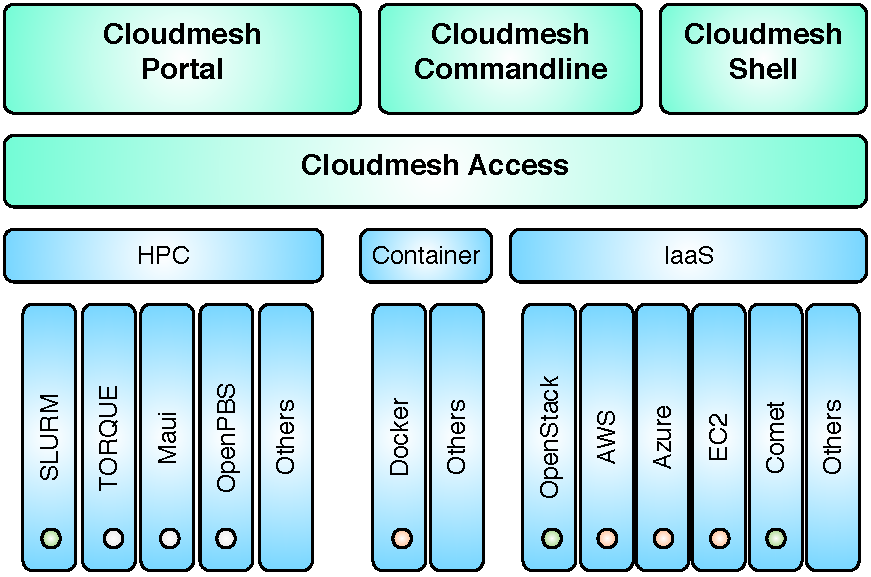
\includegraphics[width=1.0\columnwidth]{images/client/cloudmesh-arch-1.pdf}
    \caption{Cloudmesh layered architecture.}
    \label{F:arch-layer}
%\end{figure}
\bigskip
%\begin{figure}[!h]
  %\centering
    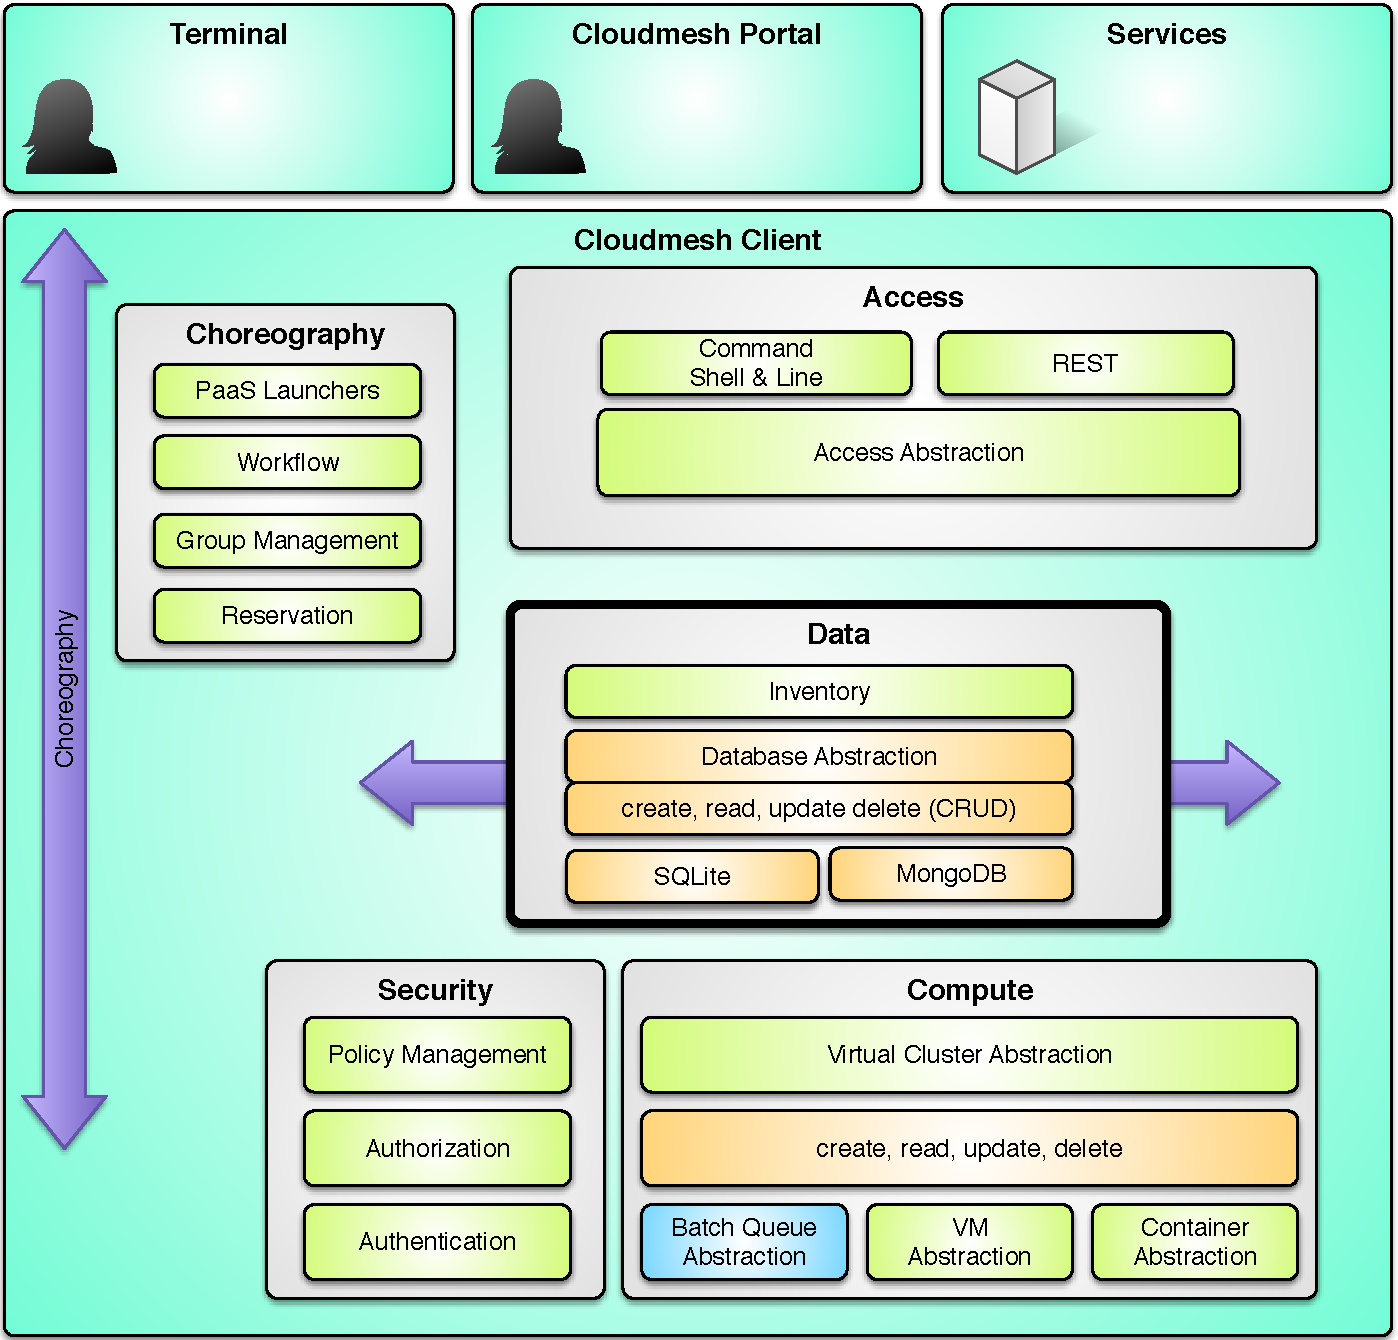
\includegraphics[width=1.0\columnwidth]{images/client/cloudmesh-arch-2.pdf}
    \caption{Cloudmesh component overview}
    \label{F:arch-component}
%\end{figure}

\bigskip

%\begin{figure}[htb]

{\tt cm comet cluster  ID}\newline -- Show the cluster details

{\tt cm comet start ID vm-ID-[0-3] --walltime=6h}\newline -- Boot 3 nodes for 6 hours

{\tt cm comet iso attach image.iso ID vm-ID-3}\newline -- Attach an iso image

{\tt cm comet power on ID vm-ID-0}\newline -- Power on node 0

{\tt cm comet console ID vm-ID-0}\newline
-- open the console for the node

\caption{Example Comet client commands}
\label{F:commands}
\end{figure}


\parindent 0pt { \bf State Caching.} Cloudmesh contains necessary state
about the resource and environment that a user may want to use.  The
information is managed in a database abstraction that would allow
storing the data in a variety of databases such as SQL and MongoDB. At
this time we have chosen SQLite to be the default database as it does
not require any additional setup and is universally available on all
operating systems without change. Previously we also provided a
MongoDB based backend system, but for the \Comet~client it is
beneficial to interact with the system without the need of additional
services.

{\parindent 0pt \bf Security Management.} For \Comet~users, it is
beneficial that access to the backend services are enabled with secure
credentials managed on the user's machine as well as with token based
service access.  This reflects best practice by many supercomputing
centers. Through abstractions integration with hosted security
services \cite{BasneyHW05} would also be possible.  However our
integration in clouds is naturally done outside such frameworks and
allows user to individually add their credentials for services such as
Azure, AWS, and other public clouds into the client easily. We have an
exploratory project in place that looks at the use of Yubikeys for
Cloudmesh Client and Cloudmesh Portal \cite{yubikey}. This will allow
an additional 2 factor authentication as part of accessing services
used by the users.  Hence, the Cloudmesh Client deals with the secured
connection and interaction by considering the appropriate interactions
with the different backends.  For the \Comet~virtualized cluster, it
handles the initial apikey retrieval, once a user is authenticated to
the nucleus service. It also handles all the subsequent calls in a
secured fashion by dealing with the messages signing, encryption and
decryption via utilizing proper libraries.

\parindent 0pt { \bf Command Shell and Command Line.} Cloudmesh contains a
command shell allowing scripts and interactive use. However we
designed the command shell in such a way that each command can also be
called from the command line reducing development and maintenance
efforts. Through the Cloudmesh database abstraction the state is
synchronized between different components.

\parindent 0pt { \bf Cloudmesh Client Portal.} Previously, we
distributed Cloudmesh with client, server, and a portal in one
package. This however turned out to be too complex to be installed for
some of our less technically skilled user communities. Thus we split up
the original Cloudmesh into multiple independent packages, such as the
{\em Cloudmesh Client} and the {\em Cloudmesh Portal}. The portal
provides currently a minimal feature set to manage virtual machines
and HPC jobs. It showcases how to integrate the client and the rest
services in more elaborated portal frameworks. We will expand upon the
existing features and make the portal more feature complete. Due to
our focus on the \Comet~community, the commandline client has an
increased development priority as it allows users to automatize
advanced {\em DevOps} workflows through scripting.

\parindent 0pt { \bf Cloudmesh Comet.} We are actively developing the
client interface for SDSC's \Comet~\cite{www-comet-user-manual}
supercomputer allowing near bare metal provisioning. The interface
reuses Cloudmesh components and technologies while interfacing with
the {\em Comet} Nucleus REST interface. Through this interplay the virtual
cluster administrators are enabled to utilize tools and services that
the they typically use to manage an on-premise bare metal cluster. As
part of this development we have developed an easy to use high level
command line interface specifically targeted to {\em Comet's\/} features. This
includes the following functionality:

\begin{itemize}
\item Configuring the nucleus service endpoint and the authentication
  tokens or keys.
\item Getting information and status of the users cluster(s), nodes,
  computesets, and other entities.
\item Power management of the cluster frontend node.
\item Request resource allocation to boot the users node(s); and release
  the resource upon completion.
\item Power management to shutoff, power on, reboot compute node(s)
  during the lifetime of the requested resource allocation.
\item Getting console access to the frontend node or a running compute
  node
\item System ISO image management. This includes listing available ISO
  images, upload new images, and attach/detach an ISO to/from one or
  more compute nodes.
\item Convenient management commands to, for example, renaming compute
  nodes either individually or in batch.
\end{itemize}

Some example commands are depicted in Figure \ref{F:commands}. The
manual page is shown in Figure \ref{F:man}.


%%% Local Variables:
%%% mode: latex
%%% TeX-master: t
%%% End:
\begin{figure}[!h]
\begin{small}
\begin{verbatim}
comet init
comet ll [CLUSTERID] [--format=FORMAT]
comet cluster [CLUSTERID][--format=FORMAT]
comet computeset [COMPUTESETID]
                 [--allocation=ALLOCATION]
                 [--cluster=CLUSTERID]
                 [--state=COMPUTESESTATE]
comet start CLUSTERID 
            [--count=NUMNODES]
            [COMPUTENODEIDS]
            [--allocation=ALLOCATION]
            [--walltime=WALLTIME]
comet terminate COMPUTESETID
comet power (on|off|reboot|reset|shutdown) 
            CLUSTERID [NODESPARAM]
comet console CLUSTERID [COMPUTENODEID]
comet iso list
comet iso upload [--isoname=ISONAME] PATHISOFILE
comet iso attach ISONAME CLUSTERID [COMPUTENODEIDS]
comet iso detach CLUSTERID [COMPUTENODEIDS]
comet node rename CLUSTERID OLDNAME NEWNAME

Options:
  --format=FORMAT         Format is either table, json, 
                          yaml, csv, rest [default: table]
  --count=NUMNODES        Number of nodes to be powered on. 
                          When this option is used, the 
                          Comet system will find a NUMNODES 
                          number of arbitrary nodes that
                          are available to boot as a 
                          computeset
  --allocation=ALLOCATION Alocation to charge 
  --walltime=WALLTIME     Walltime requested for node(s).
                          An integer followed by a unit 
                          (m,h,d,w, for minute, hour, day)
                          E.g., 3h, 2d
  --isoname=ISONAME       Name of iso image 
  --state=COMPUTESESTATE  List computeset with the given 
                          state. The state could be
                          submitted, running, completed
Arguments:
  CLUSTERID       The assigned name of a cluster, e.g. vc1
  COMPUTESETID    An integer identifier assigned to a 
                  computeset
  COMPUTENODEID   A compute node name, e.g., vm-vc1-0
                  If not provided, the requested action
                  will be taken on the frontend node of 
                  the specified cluster
  COMPUTENODEIDS  A set of compute node names in hostlist 
                  format, e.g., vm-vc1-[0-3]
                  If not provided, the requested
                  action will be taken on the frontend 
                  node of the specified cluster
  NODESPARAM      Specifying the node/nodes/computeset to
                  act on. In case of integer, will
                  be intepreted as a computesetid; in case 
                  of a hostlist format,
                  e.g., vm-vc1-[0-3], a group of nodes; 
                  or a single host is also acceptable,
                  e.g., vm-vc1-0
  ISONAME         Name of an iso image at remote server
  PATHISOFILE     The full path to the iso image file to 
                  be uploaded
\end{verbatim}
\end{small}
\caption{Cloudmesh Comet CLI Manual Page}\label{F:man}
\end{figure}



As previously mentioned, the Cloudmesh \Comet~Client deals with the
authentication to \Comet Nucleus and handles the subsequent request in
a secured fashion. It also processes the returned result from the
requests and is able to present feedback in various formats. This is
essential as it enables the user either for read in the terminal in a
human readable format such as tables or for easy scripting while being
able to access the information in YAML, JSON, or CSV. Furthermore, the
client creates data mashups from multiple information requests via the
REST interfaces in order to generate combined information views. A
good example is the Cloudmesh Client {\em cluster view} as it combines
the data from the cluster call and computeset call to generate a view
with node information, comuputeset association and status, account and
allocation data, all included in one view for easy consumption.

\parindent 0pt { \bf Cloudmesh Client Comet Python API.}
Cloudmesh Client is written in Python and provides in addition to the
commandline and command shell a Python API. This API provides high
level functionality such as data mashups that are not available in the
REST interface and provides therefor additional convenient
abstractions \cite{www-cloudmesh-client-github}.

\parindent 0pt { \bf Easy Installation.} The Cloudmesh Client is easy
to install. It is available via pip and the source code is publicly
hosted on Github \cite{www-cloudmesh-client-github}. Python 2.7
and Python 3.5 is supported.



 

%
% REMOVED IMAGES
%


\begin{comment}
\begin{figure}[!h]
  \centering
    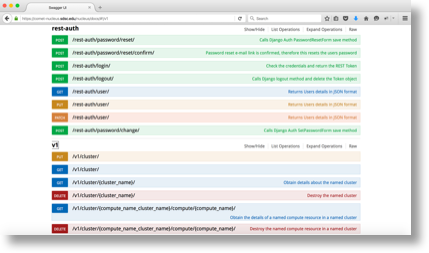
\includegraphics[width=1.0\columnwidth]{images/client/Picture1.png}
    \caption{Rest Interface}
    \label{F:1}
%\end{figure}

%\begin{figure}[htb]
  \centering
    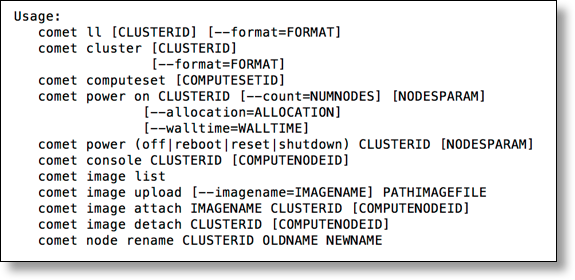
\includegraphics[width=1.0\columnwidth]{images/client/Picture2.png}
    \caption{Commandline }
    \label{F:2}
%\end{figure}

%\begin{figure}[htb]
  \centering
    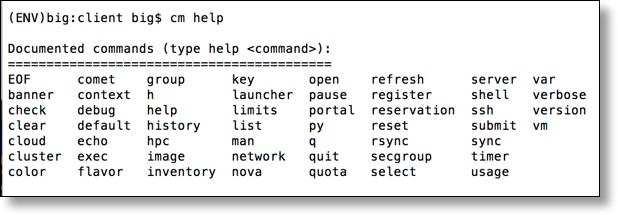
\includegraphics[width=1.0\columnwidth]{images/client/Picture3.png}
    \caption{Command Shell}
    \label{F:3}
%\end{figure}
\end{comment}






\begin{comment}
\begin{figure}[htb]
  \centering
    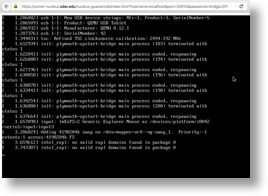
\includegraphics[width=1.0\columnwidth]{images/client/Picture4.png}
    \caption{4}
    \label{F:4}
\end{figure}
\end{comment}

\begin{comment}
%\begin{figure}[htb]
  \centering
    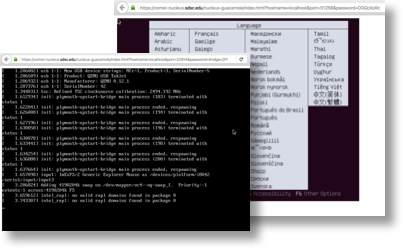
\includegraphics[width=1.0\columnwidth]{images/client/Picture5.png}
    \caption{Console}
    \label{F:5}
\end{figure}
\end{comment}


\section{Conclusifon} \label{S:conclusion}




%%%%%%%%%%%%%%%%%%%%%%%%%%%%%%%%%%%%%%%%%%%%%%%%%%%%%%%%%%%%%%%%%%%%%% 
% Acknowledgment 
%%%%%%%%%%%%%%%%%%%%%%%%%%%%%%%%%%%%%%%%%%%%%%%%%%%%%%%%%%%%%%%%%%%%%% 

\section{Acknowledgments}

 
\bibliographystyle{IEEEtran}
%\bibliography{% 
%bib/tas,%
%bib/vonlaszewski-jabref,%
%bib/vonlaszewski-new} 

\bibliography{references}


\end{document}

%%%%%%%%%%%%%%%%%%%%%%%%%%%%%%%%%%%%%%%%%%%%%%%%%%%%%%%%%%%%%%%%%%%%%%
%%%%%%%%%%%%%%%%%%%%%%%%%%%%%%%%%%%%%%%%%%%%%%%%%%%%%%%%%%%%%%%%%%%%%%
%%%%%%%%%%%%%%%%%%%%%%%%%%%%%%%%%%%%%%%%%%%%%%%%%%%%%%%%%%%%%%%%%%%%%%





\input{abstract}

\keywords{Virtual machine; Supercomputer;}


\input{introduction}

\input{dictionary}

\input{motivation}

\input{architecture}



\input{results}

\input{conclusion}

\section{Acknowledgments}

Comet is supported by NSF grant: ACI \#1341698 Gateways to Discovery:
Cyberinfrastructure for the Long Tail of Science. 

\bibliographystyle{abbrvurl}
\bibliography{references}


\end{document}
